\section{Exception Handling \verweiscpp{15}}
	\begin{minipage}[t]{7 cm}
		\subsection{Exception vs. Error}
			\begin{compactitem}
				\item Error: Abweichung zur Spezifikation ("falsch implementiert").	Errors sollten bei der Verifikation (Testen) entdeckt und eliminiert werden.
				\item Exception: abnormale (aber vorhersehbare und m�gliche) Bedingung bei der
				Programmausf�hrung.
			\end{compactitem}			
	\end{minipage}
	\hspace*{0.5cm}
	\begin{minipage}[t]{11 cm}
			\subsubsection{M�gliche Reaktionen auf Ausnahmen \verweiscpp{15.1}}
				\begin{compactitem}
				 	\item Ignorieren: Motto: Augen zu und durch, eine sehr risikoreiche Variante.
				 	\item Programmabbruch: 	Merkt immerhin, dass etwas nicht in Ordnung ist, die Reaktion ist aber unbefriedigend. Ist Exception Detection aber nicht eigentlich Exception Handling.
				 	\item Exceptioncodes (nicht Fehlercodes): Funktionen geben als R�ckgabewert, als Parameter oder global einen	Ausnahmecode an.
				\end{compactitem}
	\end{minipage} \\
	
	\subsection{Handling Strategie von System Exceptions}
		\begin{compactitem}
			\item In \lc{Java} und \lc{C\#} gelangen die System Exceptions in die Sprache, d.h. eine LowLevel Exception wird in eine Exception der Programmiersprache gemappt.
			\item Die Sprache \lc{C++} betreibt kein solches Exception Mapping, d.h. Low-Level 
			Exceptions werden nicht von \lc{C++} geworfen und k�nnen auch nicht mit
			\lc{catch(...)} abgefangen werden.
			\item Der Hauptgrund daf�r ist einmal mehr Effizienz. Wenn st�ndig Exceptions
			herumfliegen (auch wenn sie nicht abgefangen werden), dann beeintr�chtigt
			das die Performance.
			\item Einzelne Systemumgebungen betreiben dennoch Exception Mapping in \lc{C++}
			(z.B. \lc{Microsoft} in \lc{Visual C++}).
		\end{compactitem}
		
	\vspace*{-1cm}\begin{minipage}[t]{7 cm}
		\subsection{Exceptionhandling in $C++$ \verweiscpp{15.2}}
			\begin{compactitem}
				\item Exceptions werden in Form eines Objekts am Ort ihres Auftretens ausgeworfen (explizit oder auch "automatisch").
				\item Exception Handler versuchen, diese Exception-Objekte aufzufangen.
			\end{compactitem}
			
			\subsubsection{Ausl�sen (Werfen) von Ausnahmen}
				\begin{compactitem}
					\item Ausnahmen k�nnen mit dem Schl�sselwort \lc{throw} explizit ausgeworfen werden.
					\item Nach einem \lc{throw}-Befehl wird das Programm abgebrochen und beim ersten passenden umgebenden Handler fortgesetzt.
					\item Dabei werden alle lokalen Objekte wieder automatisch zerst�rt (Stack unwinding).
					\item Geworfen werden kann ein beliebiges Objekt (�blich: ein spezifisches Ausnahmeobjekt).
					\item (Ausschliesslich) innerhalb eines Exception Handlers ist auch die Form
					\lc{throw;} erlaubt. Dadurch wird die Exception an den	n�chsten Handler weitergereicht (Exception propagation).
				\end{compactitem}	
	\end{minipage}
	\hspace*{1cm}
	\begin{minipage}[t]{11 cm}
		\lstinputlisting[language=C++,tabsize=2]{code/exception_handling.cpp}
	\end{minipage} 
	
	\begin{minipage}[t]{9 cm}
		\subsubsection{Exception-Hierarchie in C++ \verweiscpp{15.4}}		 	
			Ausnahmeobjekte k�nnen beliebigen Typs sein (z.B. auch \lc{int}). Meist werden jedoch spezifische hierarchisch organisierte Ausnahmeklassen verwendet.
			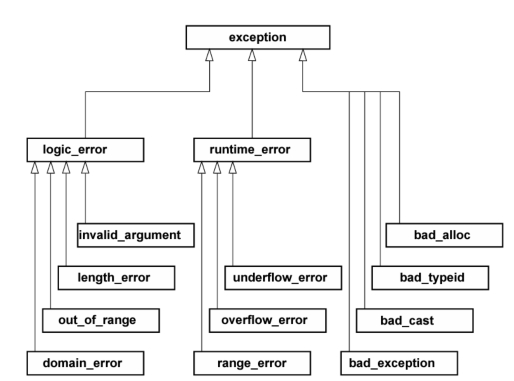
\includegraphics[width=0.69\textwidth]{pics/exception.jpg}
	\end{minipage}
	\hspace*{0.5cm}
	\begin{minipage}[t]{9 cm}
		\subsubsection{Laufzeit- vs. Logische Fehler}
			\begin{compactitem}
				\item Logische "Fehler" (logic\_error)
				\begin{compactitem}
					\item Ausnahmen im Programmablauf, die bereits zur Entwicklungszeit ihre Ursache	haben.
					\item Theoretisch k�nnten diese Ausnahmen verhindert werden.
				\end{compactitem}
				\item Laufzeit "Fehler" (runtime\_error)
				\begin{compactitem}
					\item Nicht vorhersehbare (?) Ausnahmen wie z.B. arithmetische �berl�ufe.
					\item Diese Ausnahmen treten erst zur Laufzeit auf, z.B. durch eine nicht erlaubte Benutzereingabe.
				\end{compactitem}
			\end{compactitem}
	\end{minipage} \\
	
	\begin{minipage}[t]{9 cm}
		\subsubsection{Exception Handler \verweiscpp{15.5}}
			\begin{compactitem}
				\item Ein oder mehrere Exception Handler k�nnen hintereinander definiert werden.
				\item Die einzelnen \lc{catch}-Handler m�ssen sich in den Parametern unterscheiden.
				\item Wenn eine Exception geflogen kommt, wird der erste passende Handler
				genommen. Ein passender Handler macht ein \lc{catch} auf genau diese Exception oder auf eine Basisklasse derselben.
				\item Deshalb (sehr wichtig): Der allgemeinste Handler (am meisten oben in der Hierarchie) muss als letzter definiert werden.
			\end{compactitem}
	\end{minipage}
	\hspace*{0.5cm}
	\begin{minipage}[t]{9 cm}
		\vspace*{-2.3cm}\subsubsection{Excpetions und ihre Header}
			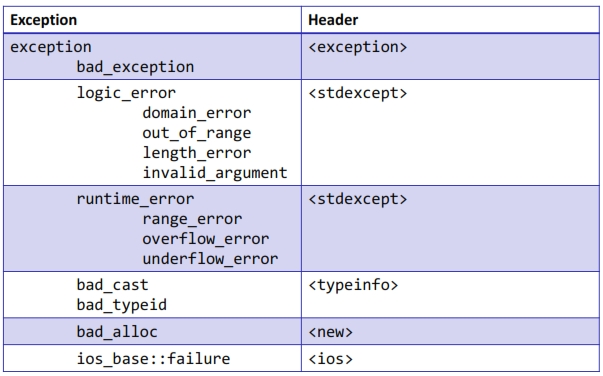
\includegraphics[width=1\textwidth]{pics/exception_header.jpg}
	\end{minipage} \\
	
		\begin{minipage}[t]{9 cm}
			\paragraph{Aufruf}
				\begin{compactitem}
					\item Wenn kein Handler passt, dann wird im Aufrufstack nach oben gesucht, ob ein	passender Handler vorhanden ist.
					\item Wenn auch dort keiner gefunden wird, dann wird die Funktion \lc{terminate()} aufgerufen.
					\item \lc{terminate()} beendet das Programm, kann aber auch selbst definiert werden.
					\item Catch all: Der folgende Handler f�ngt ausnahmslos alle Exceptions ab (und muss wenn gew�nscht deshalb immer als letzter aufgef�hrt werden):\\
					\lc{catch(...)}\\
					\lc{\{}\\
					\lc{\}}\\					
				\end{compactitem}
		\end{minipage}
		\hspace*{0.5cm}
		\begin{minipage}[t]{9 cm}				
			\paragraph{Exception Specification}
				\lc{void foo() throw(/* Liste der Exceptions */);}
				\begin{compactitem}
					\item Liste beschreibt, welche Exceptions von einem Aufrufer von \lc{foo()} erwartet werden m�ssen.
					\item Aber: garantiert auch, dass das Programm abst�rzt, wenn eine andere als die	spezifizierten Exceptions ausgeworfen wird, d.h. \lc{foo()} muss daf�r sorgen, dass wirklich nur die aufgelisteten Exceptions ausgeworfen werden.
					\item Genauer: falls eine nicht spezifizierte Exception ausgeworfen wird, dann wird die Funktion \lc{unexpected()} aufgerufen, welche �blicherweise das Programm abbricht.
					\item \lc{unexpected()} kann selbst definiert werden.
				\end{compactitem}
		\end{minipage}